\pagestyle{fancy}
\chapter{Theory}
 \label{Chap1}
    
    In this chapter we will describe the principle of superconductivity and equations that rule NIS junctions.   
        
        \section{Superconductivity}
           
            Superconductivity is a state of matter which occur at low temperature for several materials. It is a state where the material have an absolute zero resistance, so that current can run without energy losses and where the material totally excludes magnetic field and becomes perfectly diamagnetic\cite{Tinkham}. The theory of superconductivity has been established by Bardeen, Cooper and Schrieffer in 1957, and is known as the BCS Theory\cite{BCS}.
            
            The idea of the BCS theory is that electrons can pair in so-called Cooper pairs which come from the interaction between eletrons and the ion lattice, the phonons. At low temperature, electrons are slow and they tend to attract ions. These ions have a relaxation time to come back to their initial state, but during the time they are in an non-equilibrium state, they create a local positive charge (See Fig. \ref{schemaBCS}) that can attract another electron from somewhere else (10$^3$ the ion lattice caracteristic distance) in the matter. This electron is then paired with the previous one. It has the opposite wave vector and an opposite spin according to the BCS Theory. In the superconducting state, the Cooper paires form a condensate at the Fermi energy, and a consequence is the formation of a gap in the density of states (DOS).
            
            \begin{figure}
                \centering
                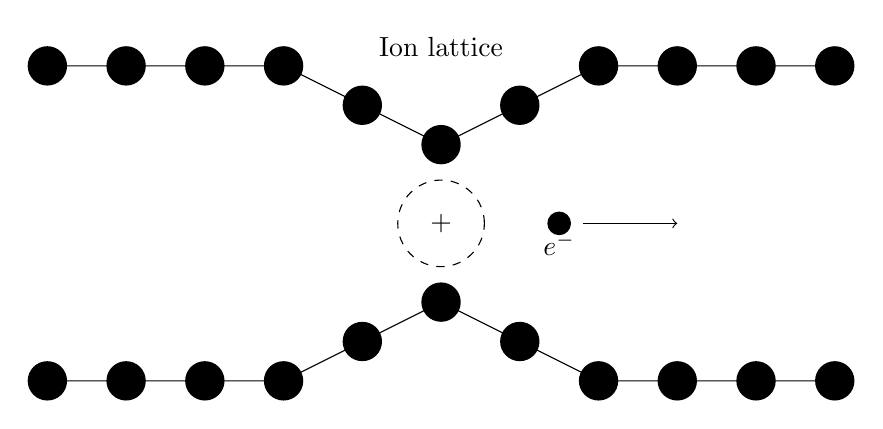
\begin{tikzpicture}
                \draw (0,0)--(3,0)--(5,1)--(7,0)--(10,0);
                \draw (0,4)--(3,4)--(5,3)--(7,4)--(10,4);
                \fill (0,0)circle(0.25);
                \fill (1,0)circle(0.25);
                \fill (2,0) circle(0.25);
                \fill (3,0) circle(0.25);
                \fill (4,0.5) circle(0.25);
                \fill (5,1) circle(0.25);
                \fill (6,0.5) circle(0.25);
                \fill (7,0) circle(0.25);
                \fill (8,0) circle(0.25);
                \fill (9,0) circle(0.25);
                \fill (10,0) circle(0.25);
                \fill (0,4) circle(0.25);
                \fill (1,4) circle(0.25);
                \fill (2,4) circle(0.25);
                \fill (3,4) circle(0.25);
                \fill (4,3.5) circle(0.25);
                \fill (5,3) circle(0.25);
                \fill (6,3.5) circle(0.25);
                \fill (7,4) circle(0.25);
                \fill (8,4) circle(0.25);
                \fill (9,4) circle(0.25);
                \fill (10,4) circle(0.25);
                \draw (5,4)node[above]{Ion lattice};
                \fill (6.5,2)circle(0.15);
                \draw [->](6.8,2)--(8,2);
                \draw (6.5,2)node[below]{$e^-$};
                \draw [dashed] (5,2)circle(0.55);
                \draw (5,2) node{$+$};
                \end{tikzpicture}
                \caption[Schematics explaining the formation of Cooper pairs]{Schematics explaining the interaction between electrons and the ion lattice. In a superconductor, the positive area attracts another electron from elsewhere in the matter}
                \label{schemaBCS}
            \end{figure}
            
            The electronic density of states follows the following rule (Eq. \ref{formuleDOS}), with N$_0$ the normal DOS and $\Delta$ the superconducting gap.
            \begin{equation}
            N(E)=\left\{ 
            \begin{array}{lr}
            \displaystyle
                N_0\dfrac{E}{\sqrt{E^2-\Delta^2}} &\text{ if } |E|>\Delta\\
                0 &\text{ if } |E|<\Delta
            \end{array}
            \right.
            \label{formuleDOS}
            \end{equation}
            
        \section[NIS Junction]{Normal Metal-Insulator-Superconductor Junction}
        
            In the case of a Normal Metal-Insulator-Superconductor (NIS) Junction, we make a contact between materials with different density of electronic states, as shown in Fig. \ref{DOSNIS0}. The DOS of a normal metal is constant at the Fermi energy and for a superconductor, it follows the previous equations. Applying a voltage will translate these densities of states. While $|eV|<\Delta$ (subgap regime), electron cannot tunnel through the insulator as there is no states available in the superconductor, but as soon as $|eV|\geqslant\Delta$ (ohmic regime), they can start to tunnel in one direction or the other depending o the sign of the bias voltage as shown in Fig. \ref{DOSNIS+} and Fig.\ref{DOSNIS-}\cite{Giaever}. It has to be noted that in principle the tunneling of a Cooper pair is possible in the region $|eV|<\Delta$, but this process is less probable (second order tunneling) and we will neglect it.
        
        \begin{figure}
        \centering
            \begin{subfigure}[t]{0.30\textwidth}
            \centering
            \begin{tikzpicture}[scale=0.49]
                \draw [domain=0.2:3] plot(\x,{1+1/\x})--++(-4,0);
                \draw [pattern=north east lines, pattern color=black] [domain=0.2:3] plot(\x,{-1-1/\x})--++(-3.9,0)--++(0,-4.66)--++(1.2,0);
                \draw [color=white,thick](-0.8,-6)--(1,-6);
                \fill (-1,6)--(-0.8,6)--(-0.8,-6)--(-1,-6)--cycle;
                \draw [pattern=north east lines, pattern color=black] (-4,-6) rectangle (-1,0);
                \draw [color=white,thick] (-1,-6)--(-4,-6)--(-4,0);
                \draw [<->] (1,0)--(1,1.33)node[midway,right]{$\Delta$};
                \draw (-4,0)--(-1,0);
                \draw [dashed](-0.8,0)--(3,0);
                \draw (3,0)node[right]{$E_F$};
                \draw (-2.5,6.5)node{N};
                \draw (-0.9,6.5)node{I};
                \draw (0.5,6.5)node{S};
                \end{tikzpicture}
                \caption{Density of States at\\$V_{bias}=0$}
                \label{DOSNIS0}
                \end{subfigure}
                ~
                \begin{subfigure}[t]{0.30\textwidth}
                \centering
                \begin{tikzpicture}[scale=0.49]
                \draw [domain=0.2:3] plot(\x,{1+1/\x})--++(-4,0);
               \draw [pattern=north east lines, pattern color=black] [domain=0.2:3] plot(\x,{-1-1/\x})--++(-3.9,0)--++(0,-4.66)--++(1.2,0);
                \draw [color=white,thick](-0.8,-6)--(1,-6);
                \fill (-1,6)--(-0.8,6)--(-0.8,-6)--(-1,-6)--cycle;
                \draw [pattern=north east lines, pattern color=black] (-4,-6) rectangle (-1,2.3);
                \draw [color=white,thick] (-1,-6)--(-4,-6)--(-4,2.3);
                \draw [<->](-4.1,0)--(-4.1,2.3)node[midway,left]{$V_{bias}$};
                \draw [->] (-0.8,1.9) arc (90:45:1) node[near end,above]{$e^-$};
                \draw [dashed](-0.8,0)--(3,0);
                \draw (-2.5,6.5)node{N};
                \draw (-0.9,6.5)node{I};
                \draw (0.5,6.5)node{S};
                \end{tikzpicture}
                \caption{Density of States at\\$eV_{bias}>\Delta$}
                \label{DOSNIS+}
                \end{subfigure}
                ~
                \begin{subfigure}[t]{0.30\textwidth}
                \centering
                \begin{tikzpicture}[scale=0.49]
                \draw [domain=0.2:3] plot(\x,{1+1/\x})--++(-4,0);
               \draw [pattern=north east lines, pattern color=black] [domain=0.2:3] plot(\x,{-1-1/\x})--++(-3.9,0)--++(0,-4.66)--++(1.2,0);
                \draw [color=white,thick](-0.8,-6)--(1,-6);
                \fill (-1,6)--(-0.8,6)--(-0.8,-6)--(-1,-6)--cycle;
                \draw [pattern=north east lines, pattern color=black] (-4,-6) rectangle (-1,-2);
                \draw [color=white,thick] (-1,-6)--(-4,-6)--(-4,-2);
                \draw [<->](-4.1,0)--(-4.1,-2)node[midway,left]{$V_{bias}$};
                \draw [->] (-1,-1.5) arc(90:130:1)node[near end, above]{$e^-$};
                \draw [dashed](-0.8,0)--(3,0);
                \draw (-2.5,6.5)node{N};
                \draw (-0.9,6.5)node{I};
                \draw (0.5,6.5)node{S};
                \end{tikzpicture}
                \caption{Density of States at\\$eV_{bias}<-\Delta$}
                \label{DOSNIS-}
                \end{subfigure}
                \caption{Density of states for different $V_{bias}$ for a NIS junction}
                \label{DOSNIS}
        \end{figure}
        
        The current that crosses the NIS junctions is where $f$ is the Fermi-Dirac distribution, and $g$ the density of states.
        \begin{equation}
            \displaystyle
            I(V)=\dfrac{1}{2e}\int d\varepsilon g(\varepsilon)[f(\varepsilon-eV)-f(\varepsilon+eV)]
        \end{equation}
        
        \section{Leakage current}
        
        In practice, the junctions are not perfect and electron tunneling can be induced by some impurities or by interaction with photon. To take into account these unwanted tunneling processes, we introduce the Dynes density of states \cite{Dynes_DOS}. It is a broadening of the DOS written in the BCS theory with a linewidth parameter $\Gamma$ :
        
        \begin{equation}
            N=Re\left(\dfrac{|E|+i\Gamma}{\sqrt{(E+i\Gamma)^2-\Delta^2}}\right)
            \label{DynesDOS}
        \end{equation}        
        
        This new DOS induces a small durrent in the subgap regime.So there can be tunneling within the gap since the DOS in not equal to zero, however very limited. The resulting current is called leakage current and shows, among other things, the defaults of the junction. The leakage is defined as the ratio between the resistance in the ohmic regime ($R$) and the resistance in the subgap regime ($R_{leak}$). A junction is generally considered as good if :
        
        \[\dfrac{R}{R_{leak}}<10^{-4}\]


        
        
        
